\documentclass[11pt,a4paper]{article}
%%%%%%%%%%%%%%%%%%%%%%%%% PACKAGE starts HERE %%%%%%%%%%%%%%%%%%%%%%%%
\usepackage{graphicx}
\usepackage{caption}
% \usepackage{microtype}
\captionsetup[table]{name=Tabel}
\captionsetup[figure]{name=Gambar}
\usepackage{tabulary}
% \usepackage{minted}
\usepackage{fancyhdr}
\usepackage{placeins}
\usepackage{graphicx}
\usepackage[all]{xy}
\usepackage{tikz}
\usepackage{verbatim}
\usepackage[left=2cm,right=2cm,top=3cm,bottom=2.5cm]{geometry}
\usepackage{hyperref}
\hypersetup{
    colorlinks,
    linkcolor={red!50!black},
    citecolor={blue!50!black},
    urlcolor={blue!80!black}
}
\usepackage{caption}
\usepackage{subcaption}
\usepackage{multirow}
\usepackage{psfrag}
\usepackage[T1]{fontenc}
\usepackage[scaled]{beramono}
\usepackage{listings}
\usepackage{xcolor}

\definecolor{codegreen}{rgb}{0,0.6,0}
\definecolor{codegray}{rgb}{0.5,0.5,0.5}
\definecolor{codepurple}{rgb}{0.58,0,0.82}
\definecolor{backcolour}{rgb}{0.95,0.95,0.92}
\definecolor{LightGray}{gray}{0.9}

\lstdefinestyle{mystyle}{
	backgroundcolor=\color{backcolour},
	commentstyle=\color{green},
	keywordstyle=\color{codegreen},
	numberstyle=\tiny\color{codegray},
	stringstyle=\color{codepurple},
	basicstyle=\ttfamily\footnotesize,
	breakatwhitespace=false,
	breaklines=true,
	captionpos=b,
	keepspaces=true,
	numbers=left,
	numbersep=5pt,
	showspaces=false,
	showstringspaces=false,
	showtabs=false,
	tabsize=2
}
\lstset{style=mystyle}
\renewcommand{\lstlistingname}{Kode}
%%%%%%%%%%%%%%%%%%%%%%%%% PACKAGE ends HERE %%%%%%%%%%%%%%%%%%%%%%%%

%%%%%%%%%%%%%%%%%%%%%%%%% Data Diri %%%%%%%%%%%%%%%%%%%%%%%%
\newcommand{\student}{\textbf{Ferdana Al-Hakim}}
\newcommand{\course}{\textbf{Sistem/Teknologi Multimedia (IF25-40305)}}
\newcommand{\assignment}{\textbf{Final Project}}

\usepackage{fancyhdr}
\pagestyle{fancy}
\lhead{Ferdana Al-Hakim}
\rhead{\thepage}
\cfoot{\textbf{HandBeats: Gesture Rhythm Game}}
\renewcommand{\headrulewidth}{0.4pt}
\renewcommand{\footrulewidth}{0.4pt}
\setlength\headheight{14pt}

%%%%%%%%%%%%%%%%%%%%%%%%%%%%%%%%%%%%%%%%%%%%%%%%%%%%%%%%%%%%%%%
\begin{document}
\thispagestyle{empty}
\begin{center}
	\includegraphics[scale = 0.15]{ifitera-header.png}
	\vspace{0.1cm}
\end{center}
\noindent
\rule{17cm}{0.2cm}\\[0.3cm]
Nama: \student \hfill Tugas Ke: \assignment\\[0.1cm]
Mata Kuliah: \course \hfill Tanggal: Desember 2024\\
\rule{17cm}{0.05cm}
\vspace{0.5cm}

\begin{center}
    \Large\textbf{HANDBEATS: GESTURE RHYTHM GAME}\\
    \large\textit{Game Ritme Berbasis Deteksi Gesture Tangan}
\end{center}

%%%%%%%%%%%%%%%%%%%%%%%%%%%%%%%%%%%%%%%%%%%%% BODY DOCUMENT %%%%%%%%%%%%%%%%%%%%%%%%%%%%%%%%%%%%%%%%%%%%%
\section{Pendahuluan}

HandBeats adalah game interaktif berbasis kamera yang mengintegrasikan tiga komponen pemrosesan multimedia: \textit{image processing}, \textit{video processing}, dan \textit{audio processing}. Game ini menampilkan zona instrumen musik seperti "Kick", "Snare", dan "Hi-Hat" di layar, di mana pemain harus mengetuk area tersebut menggunakan gesture tangan dengan timing yang tepat mengikuti irama musik.

\subsection{Latar Belakang}

Perkembangan teknologi \textit{computer vision} dan \textit{machine learning} memungkinkan deteksi gesture tangan secara real-time dengan akurasi tinggi. Teknologi ini dapat dimanfaatkan untuk menciptakan pengalaman interaktif yang menarik dalam bentuk rhythm game yang tidak memerlukan perangkat input tambahan selain webcam.

\subsection{Tujuan}

Tujuan dari pembuatan project ini adalah:
\begin{itemize}
    \item Mengimplementasikan pemrosesan image untuk deteksi tangan menggunakan MediaPipe Hands
    \item Mengintegrasikan pemrosesan video real-time dengan overlay grafis game
    \item Menerapkan pemrosesan audio untuk musik loop seamless dan sound effects
    \item Menciptakan gameplay yang responsif dengan sistem scoring dan feedback visual
\end{itemize}

\section{Komponen Multimedia}

Project HandBeats mengintegrasikan tiga komponen utama pemrosesan multimedia yang bekerja secara bersamaan untuk menciptakan pengalaman bermain yang interaktif.

\subsection{Image Processing}

Komponen image processing bertanggung jawab untuk mendeteksi dan melacak posisi tangan pemain secara real-time menggunakan MediaPipe Hands.

\subsubsection{MediaPipe Hands Detection}

MediaPipe Hands adalah solusi machine learning untuk deteksi tangan yang dapat mendeteksi hingga 21 landmark pada setiap tangan. Implementasi pada HandBeats menggunakan confidence threshold 0.7 untuk memastikan deteksi yang akurat.

\begin{lstlisting}[language=Python, caption=Inisialisasi MediaPipe Hands,label={code:mediapipe}]
class HandTracker:
    def __init__(self):
        self.mp_hands = mp.solutions.hands
        self.hands = self.mp_hands.Hands(
            static_image_mode=False,
            max_num_hands=2,
            min_detection_confidence=0.7,
            min_tracking_confidence=0.7
        )
        self.mp_drawing = mp.solutions.drawing_utils
\end{lstlisting}

\subsubsection{Bounding Box Calculation}

Setelah landmark terdeteksi, sistem menghitung bounding box untuk setiap tangan yang digunakan dalam collision detection dengan zona target.

\begin{lstlisting}[language=Python, caption=Kalkulasi Bounding Box Tangan,label={code:bbox}]
def calculate_hand_bbox(self, hand_landmarks, width, height):
    x_coords = [lm.x for lm in hand_landmarks.landmark]
    y_coords = [lm.y for lm in hand_landmarks.landmark]

    min_x = int(min(x_coords) * width)
    max_x = int(max(x_coords) * width)
    min_y = int(min(y_coords) * height)
    max_y = int(max(y_coords) * height)

    return {
        'x': min_x,
        'y': min_y,
        'width': max_x - min_x,
        'height': max_y - min_y
    }
\end{lstlisting}

\subsection{Video Processing}

Video processing menangani capture frame dari webcam, konversi color space, dan rendering overlay grafis game ke layar.

\subsubsection{Camera Capture}

Sistem menggunakan OpenCV untuk capture video dari webcam dengan resolusi 1280x720 (HD 720p) untuk memastikan kualitas deteksi yang optimal.

\begin{lstlisting}[language=Python, caption=Inisialisasi Kamera,label={code:camera}]
self.camera = cv2.VideoCapture(0)
self.camera.set(cv2.CAP_PROP_FRAME_WIDTH, 1280)
self.camera.set(cv2.CAP_PROP_FRAME_HEIGHT, 720)
\end{lstlisting}

\subsubsection{Frame Processing dan Overlay}

Setiap frame video yang ditangkap diproses untuk deteksi tangan, kemudian di-composite dengan elemen grafis game seperti falling objects, score, dan visual feedback.

\begin{lstlisting}[language=Python, caption=Pemrosesan Video Frame,label={code:videoprocess}]
def _render_camera_feed(self, frame):
    # Konversi BGR ke RGB
    frame_rgb = cv2.cvtColor(frame, cv2.COLOR_BGR2RGB)

    # Resize dengan aspect fill
    scale = max(target_width / src_w, target_height / src_h)
    new_w = int(src_w * scale)
    new_h = int(src_h * scale)

    frame_resized = cv2.resize(frame_rgb, (new_w, new_h))

    # Center crop
    frame_cropped = frame_resized[crop_y:crop_y + target_height,
                                  crop_x:crop_x + target_width]

    # Convert ke pygame surface
    frame_transposed = np.transpose(frame_cropped, (1, 0, 2))
    frame_surface = pygame.surfarray.make_surface(frame_transposed)

    self.screen.blit(frame_surface, (0, 0))
\end{lstlisting}

\subsection{Audio Processing}

Audio processing mengelola musik background loop dan sound effects instrumen yang dimainkan saat pemain berhasil mengenai target.

\subsubsection{Seamless Music Looping}

Musik background di-loop secara seamless tanpa jeda menggunakan pygame.mixer dengan beat duration 9 detik.

\begin{lstlisting}[language=Python, caption=Music Looping,label={code:audioloop}]
def play_main_beat(self, loops=-1):
    if not self.music_playing:
        pygame.mixer.music.play(loops)  # -1 untuk infinite loop
        self.music_playing = True
        print("Main beat started (looping)")
\end{lstlisting}

\subsubsection{Polyphonic Sound Effects}

Sistem audio mendukung polyphonic playback, memungkinkan multiple sound effects dimainkan bersamaan saat pemain mengenai multiple targets secara simultan.

\begin{lstlisting}[language=Python, caption=Instrument Sound Playback,label={code:soundfx}]
def play_instrument(self, instrument: str):
    if instrument in self.sounds and self.sounds[instrument]:
        self.sounds[instrument].play()

def play_hit_sound(self, hit_type: str = 'good'):
    volume = {
        'perfect': 1.0,
        'good': 0.8,
        'ok': 0.6
    }.get(hit_type, 0.8)

    sound = self.sounds['hit']
    sound.set_volume(volume)
    sound.play()
\end{lstlisting}

\section{Implementasi Sistem}

\subsection{Arsitektur Sistem}

HandBeats dibangun dengan arsitektur modular yang memisahkan setiap komponen ke dalam module terpisah untuk maintainability dan scalability. Struktur project dapat dilihat pada kode \ref{code:structure}.

\begin{lstlisting}[language=bash, caption=Struktur Project,label={code:structure}]
handbeats-rhythm-game/
├── main.py                  # Entry point
├── config/
│   ├── constants.py         # Konstanta warna, zona, path
│   ├── settings.py          # Pengaturan difficulty
│   └── beatmap.py           # Generator pattern
├── src/
│   ├── game_manager.py      # Orchestrator utama
│   ├── audio_manager.py     # Audio processing
│   ├── hand_tracker.py      # Image processing
│   ├── lane.py              # Target zones
│   ├── falling_object.py    # Rhythm notes
│   ├── collision.py         # Hit detection
│   └── score_manager.py     # Scoring system
├── ui/
│   ├── menu_screen.py       # Main menu
│   ├── game_screen.py       # Game UI
│   └── result_screen.py     # Result stats
└── assets/
    ├── audio/               # Music dan SFX
    └── image/               # Icon instrumen
\end{lstlisting}

\subsection{Alur Sistem}

Alur kerja sistem HandBeats dapat dilihat pada flowchart di Gambar \ref{fig:flowchart}. Sistem dimulai dari menu pemilihan difficulty, kemudian melakukan inisialisasi komponen multimedia, masuk ke game loop utama, dan diakhiri dengan layar hasil.

\begin{figure}[h]
    \centering
    \includegraphics[width=1\textwidth]{alur.png}
    \caption{Flowchart Alur Sistem HandBeats}
    \label{fig:flowchart}
\end{figure}

\subsection{Game Loop}

Game loop merupakan inti dari sistem yang mengintegrasikan ketiga komponen multimedia secara real-time.

\begin{lstlisting}[language=Python, caption=Main Game Loop,label={code:gameloop}]
def update_gameplay(self, dt: float):
    self.game_time += dt

    # VIDEO PROCESSING: Capture frame
    ret, frame = self.camera.read()

    # IMAGE PROCESSING: Detect hands
    frame, hand_results, face_results = self.hand_tracker.process_frame(frame)

    # Get positions untuk collision
    fingertip_positions = self.hand_tracker.get_fingertip_positions(
        hand_results, SCREEN_WIDTH, SCREEN_HEIGHT
    )

    # Calculate velocities untuk gesture detection
    fingertip_velocities = self.hand_tracker.calculate_velocity(
        fingertip_positions,
        self.hand_tracker.prev_fingertip_positions
    )

    # Update lanes dengan velocity check
    active_lanes = self.lane_manager.check_collisions_with_velocity(
        fingertip_positions,
        chin_position,
        fingertip_velocities,
        chin_velocity,
        self.hand_tracker.velocity_threshold
    )

    # COLLISION DETECTION
    objects_in_zone = self.falling_objects.get_objects_in_hit_zone()
    hit_results = self.collision_detector.check_multiple_objects(
        objects_in_zone, active_lanes
    )

    # Process hit results
    for hit_result in hit_results:
        self.score_manager.add_hit(hit_result)

        # AUDIO PROCESSING: Play sounds
        self.audio_manager.play_hit_sound(hit_result.rating.lower())
        self.audio_manager.play_instrument(hit_result.instrument)
\end{lstlisting}

\subsection{Collision Detection}

Sistem collision detection menggunakan velocity-based gesture recognition untuk mencegah "idle farming" - pemain harus benar-benar melakukan gerakan cepat untuk mengenai target.

\begin{lstlisting}[language=Python, caption=Velocity-Based Collision Detection,label={code:collision}]
def check_collisions_with_velocity(self, fingertip_positions,
                                   fingertip_velocities,
                                   velocity_threshold):
    active_lanes = {}

    for lane in self.lanes:
        lane_active = False

        for hand_label, fingertip_zone in fingertip_positions.items():
            if lane.check_hand_collision(fingertip_zone):
                # Check velocity - harus bergerak cukup cepat!
                if (hand_label in fingertip_velocities and
                    fingertip_velocities[hand_label] >= velocity_threshold):
                    lane_active = True
                    active_lanes[lane.instrument] = hand_label
                    break

        lane.activate(lane_active)

    return active_lanes
\end{lstlisting}

\subsection{Difficulty System}

Game menyediakan tiga tingkat kesulitan yang mempengaruhi kecepatan falling objects, timing window, dan kompleksitas pattern.

\begin{lstlisting}[language=Python, caption=Difficulty Settings,label={code:difficulty}]
EASY = {
    'falling_speed': 5.0,
    'pattern_type': 'simple',
    'perfect_window': 120,  # ±120ms
    'good_window': 200,     # ±200ms
    'ok_window': 300        # ±300ms
}

MEDIUM = {
    'falling_speed': 7.0,
    'pattern_type': 'smart',
    'perfect_window': 80,
    'good_window': 150,
    'ok_window': 230
}

HARD = {
    'falling_speed': 9.5,
    'pattern_type': 'complex',
    'perfect_window': 60,
    'good_window': 120,
    'ok_window': 180
}
\end{lstlisting}

\section{User Interface}

\subsection{Menu Screen}

Menu screen menampilkan pilihan difficulty dengan visual yang menarik dan mudah dipahami. Background menggunakan pixel art style dengan overlay semi-transparent untuk keterbacaan teks yang optimal (Gambar \ref{fig:menu}).

\begin{figure}[h]
    \centering
    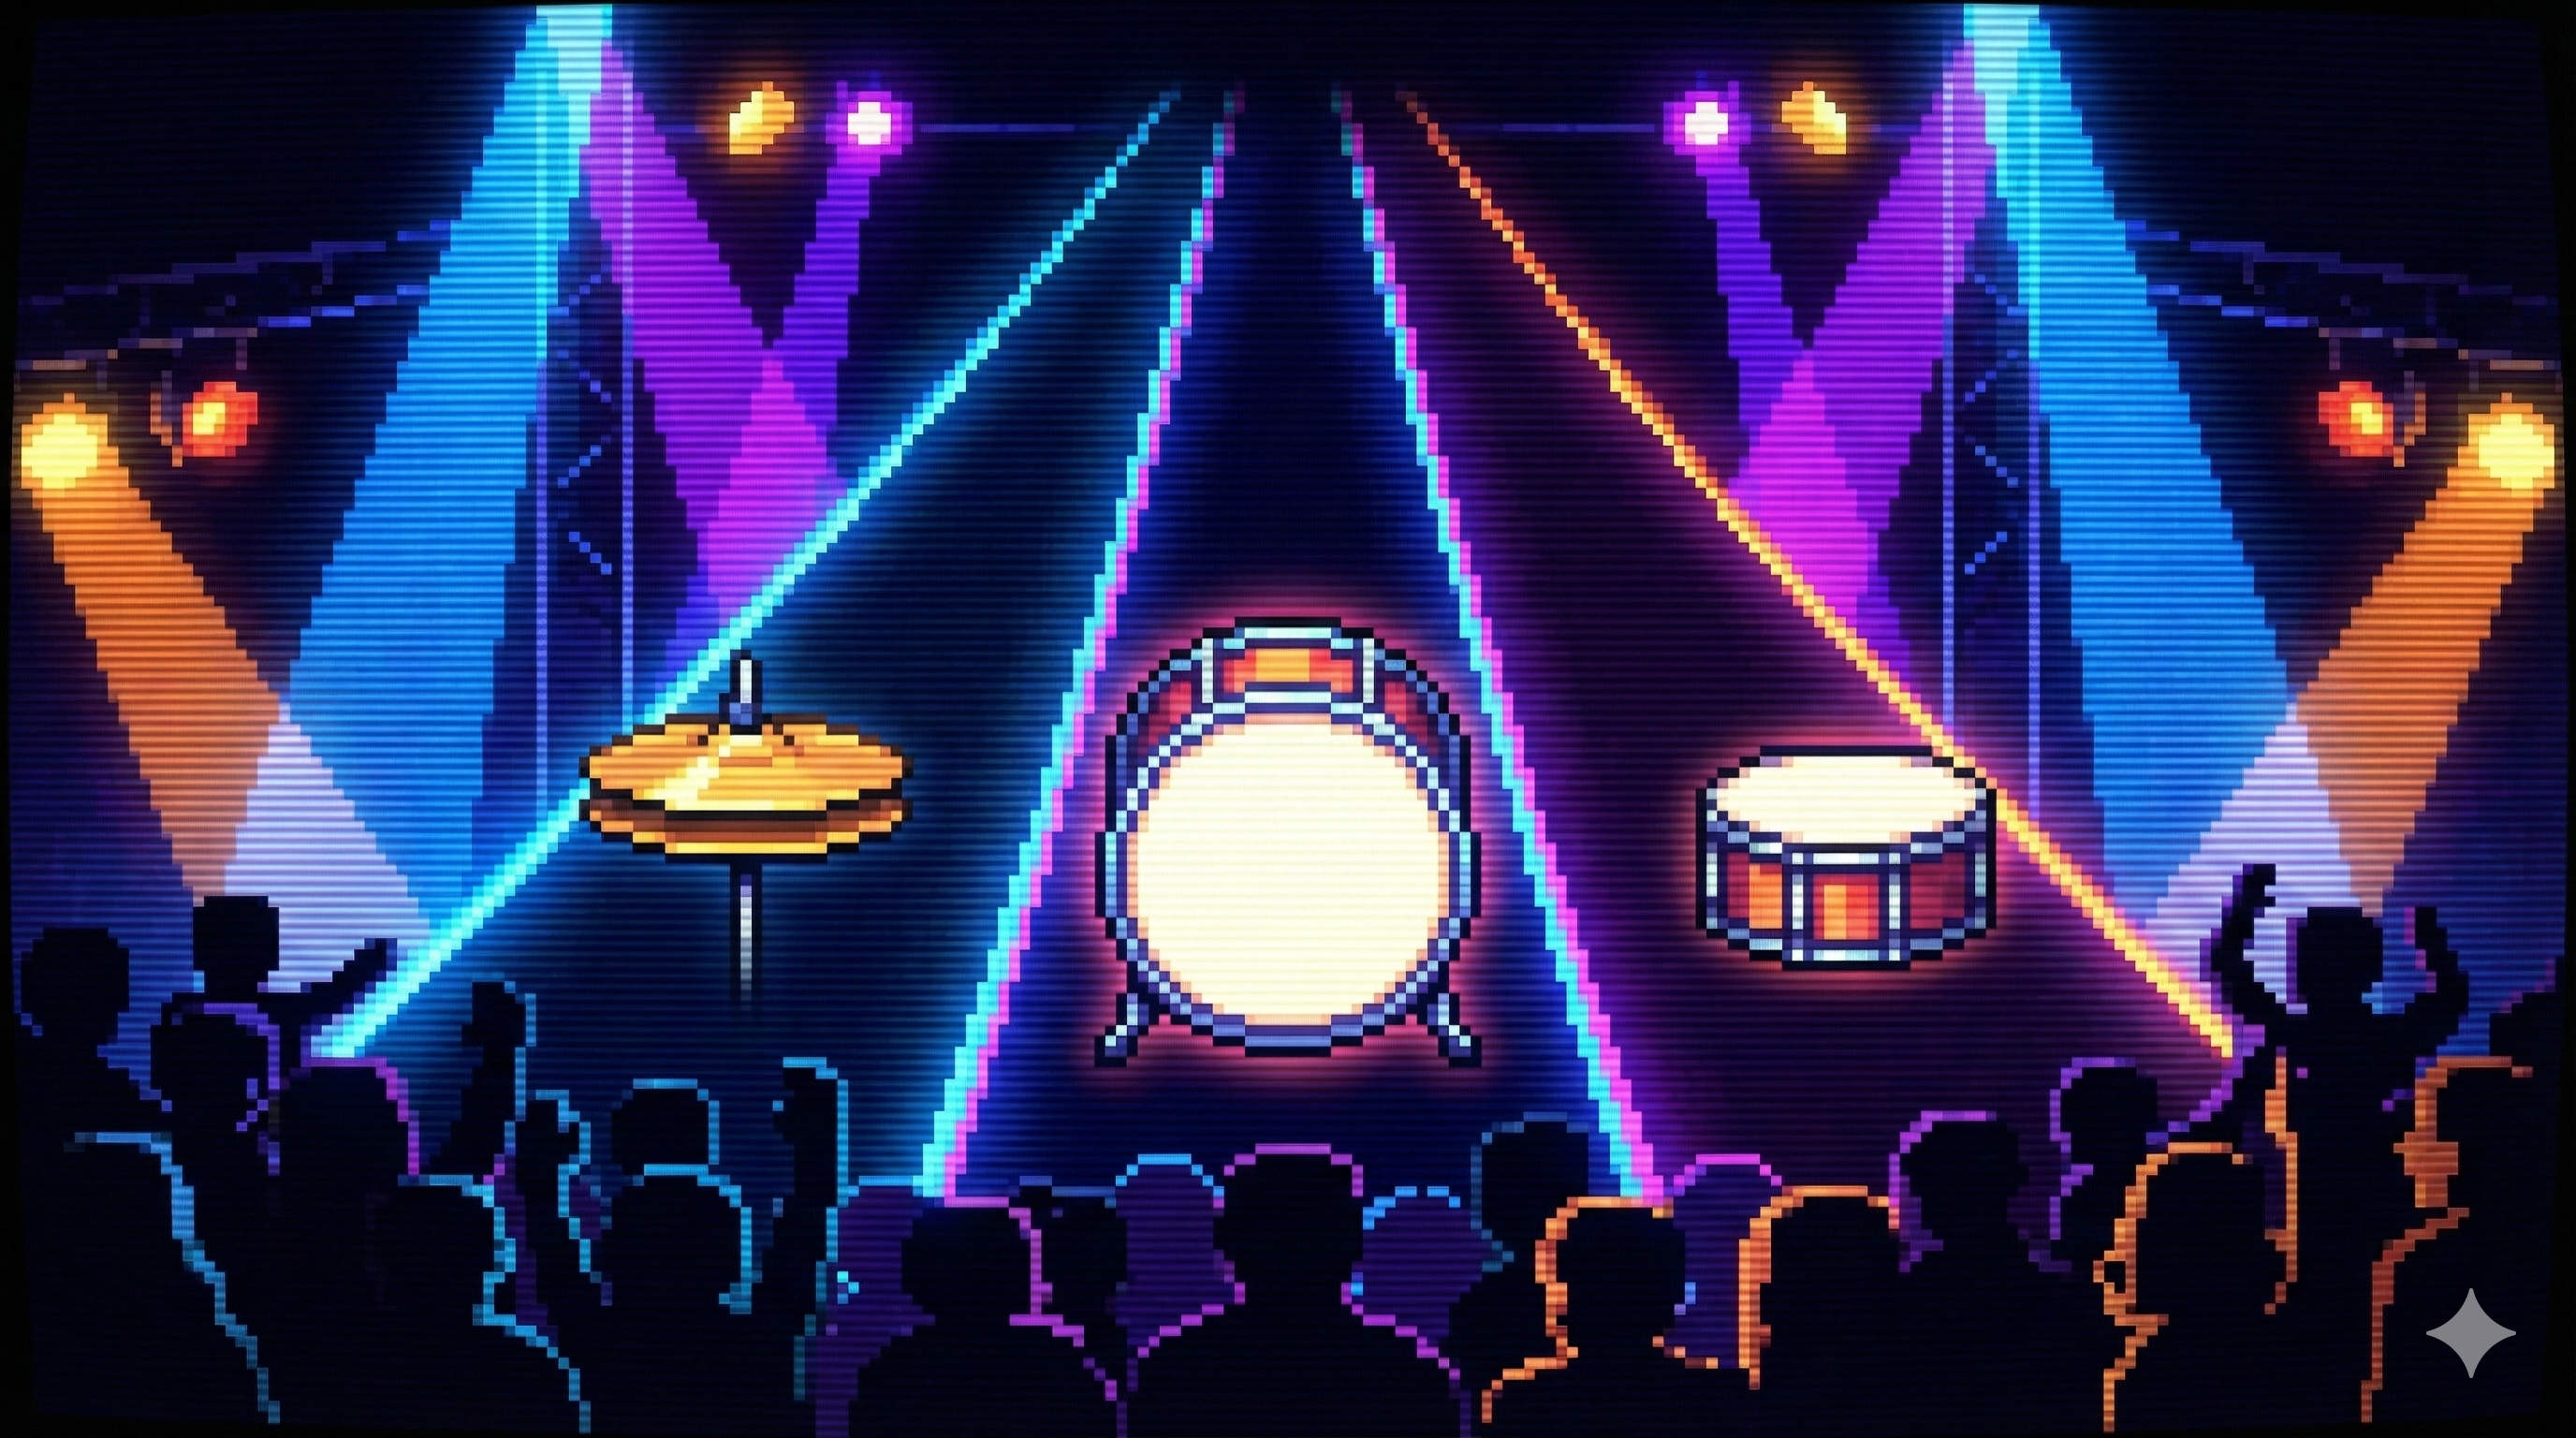
\includegraphics[width=0.85\textwidth]{menu.png}
    \caption{Menu Screen dengan Difficulty Selection}
    \label{fig:menu}
\end{figure}

\subsection{Gameplay Screen}

Layar gameplay menampilkan video feed dari kamera sebagai background fullscreen dengan overlay elemen game seperti score, combo, timer, falling objects, dan visual feedback (Gambar \ref{fig:gameplay}).

\begin{figure}[h]
    \centering
    \includegraphics[width=0.85\textwidth]{gamelay.png}
    \caption{Gameplay Screen dengan Video Overlay}
    \label{fig:gameplay}
\end{figure}

Elemen-elemen UI pada gameplay:
\begin{itemize}
    \item \textbf{Score}: Menampilkan skor saat ini di pojok kiri atas
    \item \textbf{Combo}: Menampilkan combo count di tengah atas dengan multiplier
    \item \textbf{Timer}: Countdown waktu permainan di pojok kanan atas
    \item \textbf{Lanes}: Tiga zona target (Kick, Snare, Hi-Hat) dengan icon instrumen
    \item \textbf{Falling Objects}: Notes yang jatuh dari atas ke zona target
    \item \textbf{Hand Indicators}: Lingkaran biru/oranye menunjukkan posisi fingertip
\end{itemize}

\subsection{Result Screen}

Result screen menampilkan statistik lengkap performa pemain setelah game berakhir, termasuk score, accuracy, rank, combo, dan breakdown hit counts (Gambar \ref{fig:result}).

\begin{figure}[h]
    \centering
    \includegraphics[width=0.85\textwidth]{score.png}
    \caption{Result Screen dengan Performance Stats}
    \label{fig:result}
\end{figure}

\section{Sistem Scoring}

\subsection{Timing Windows}

Sistem scoring menggunakan timing windows untuk menentukan akurasi hit. Semakin dekat timing dengan target, semakin tinggi poin yang didapat.

\begin{table}[h]
\caption{Timing Windows dan Point Values}
\label{tab:scoring}
\centering
\begin{tabular}{|l|c|c|c|}
\hline
\textbf{Rating} & \textbf{Easy} & \textbf{Medium} & \textbf{Hard} \\ \hline
PERFECT & ±120ms (100 pts) & ±80ms (100 pts) & ±60ms (100 pts) \\ \hline
GOOD & ±200ms (50 pts) & ±150ms (50 pts) & ±120ms (50 pts) \\ \hline
OK & ±300ms (25 pts) & ±230ms (25 pts) & ±180ms (25 pts) \\ \hline
MISS & Outside window (0 pts) & Outside window (0 pts) & Outside window (0 pts) \\ \hline
\end{tabular}
\end{table}

\subsection{Combo Multiplier}

Sistem combo memberikan multiplier bonus untuk consecutive hits yang berhasil:
\begin{itemize}
    \item 10x combo: 1.2x multiplier
    \item 20x combo: 1.5x multiplier
    \item 30x combo: 2.0x multiplier
    \item 50x combo: 2.5x multiplier
\end{itemize}

\subsection{Ranking System}

Setelah game berakhir, sistem memberikan rank berdasarkan accuracy:
\begin{itemize}
    \item S Rank: 95\% - 100\%
    \item A Rank: 85\% - 94\%
    \item B Rank: 75\% - 84\%
    \item C Rank: 65\% - 74\%
    \item D Rank: < 65\%
\end{itemize}

\section{Teknologi dan Tools}

\subsection{Library dan Framework}

Project ini menggunakan beberapa library Python untuk implementasi:
\begin{itemize}
    \item \textbf{Pygame}: Game engine dan audio processing
    \item \textbf{OpenCV}: Video capture dan frame processing
    \item \textbf{MediaPipe}: Hand detection dan tracking
    \item \textbf{NumPy}: Array manipulation untuk image processing
\end{itemize}

\subsection{Development Tools}

Tools yang digunakan dalam development:
\begin{itemize}
    \item \textbf{Python 3.11}: Programming language
    \item \textbf{VS Code}: Code editor
    \item \textbf{Git}: Version control
    \item \textbf{Draw.io}: Flowchart design
\end{itemize}

\section{Kesimpulan}

HandBeats berhasil mengintegrasikan tiga komponen multimedia (image, video, audio processing) menjadi sebuah rhythm game interaktif yang responsif dan engaging. Penggunaan MediaPipe untuk hand detection memberikan akurasi tinggi, sementara sistem collision detection berbasis velocity memastikan gameplay yang fair dan challenging.

\subsection{Pencapaian}

\begin{itemize}
    \item Implementasi real-time hand tracking dengan MediaPipe
    \item Integrasi seamless video overlay dengan gameplay elements
    \item Audio system dengan polyphonic playback dan infinite looping
    \item Tiga tingkat kesulitan dengan dynamic pattern generation
    \item Scoring system dengan combo multiplier dan ranking
\end{itemize}

\subsection{Pengembangan Masa Depan}

Beberapa fitur yang dapat dikembangkan:
\begin{itemize}
    \item Online leaderboard untuk competitive play
    \item Custom song import dengan auto-beatmap generation
    \item Multiplayer mode untuk head-to-head competition
    \item Achievement system dan progression tracking
    \item Mobile platform support menggunakan Kivy atau similar framework
\end{itemize}

\section*{Lampiran}

\subsection*{AI Assistant Tools}

Dalam pengembangan project ini, beberapa AI assistant digunakan untuk membantu problem solving, code optimization, dan debugging:

\begin{itemize}
    \item \textbf{ChatGPT}: Untuk konsultasi arsitektur sistem, debugging, dan optimisasi algoritma
    \begin{itemize}
        \item Link: \href{https://chatgpt.com/share/68ff6cbb-d63c-800f-871e-9593a1298534}{https://chatgpt.com/share/68ff6cbb-d63c-800f-871e-9593a1298534}
    \end{itemize}

    \item \textbf{Google Gemini}: Untuk optimisasi collision detection dan performance tuning
    \begin{itemize}
        \item Link: \href{https://gemini.google.com/share/beadc25d28a9}{https://gemini.google.com/share/beadc25d28a9}
    \end{itemize}

    \item \textbf{Claude Code}: Untuk code refactoring, documentation, dan implementation assistance
\end{itemize}

\subsection*{Asset Credits}

\begin{itemize}
    \item Background Music: Original composition (9-second loop, 120 BPM)
    \item Sound Effects: \href{https://pixabay.com/}{Pixabay Free Sound Library}
    \begin{itemize}
        \item Kick drum sample
        \item Snare drum sample
        \item Hi-hat sample
    \end{itemize}
    \item Menu Background: Custom pixel art design
    \item Instrument Icons: Custom designed PNG assets
\end{itemize}

\subsection*{Repository}

Source code project HandBeats tersedia secara lengkap di GitHub:

\href{https://github.com/luciferdana/handbeats-rhythm-game}{https://github.com/luciferdana/handbeats-rhythm-game}

\end{document}
